\documentclass[a4paper,12pt]{article} 
\usepackage[T2A]{fontenc}			
\usepackage[utf8]{inputenc}			
\usepackage[english,russian]{babel}
\usepackage{float}
\usepackage{amsmath,amsfonts,amssymb,amsthm,mathrsfs,mathtools} 
\usepackage{cancel}
\usepackage{multirow}
\usepackage[colorlinks, linkcolor = blue]{hyperref}
\usepackage{upgreek}
\usepackage[left=2cm,right=2cm,top=2cm,bottom=3cm,bindingoffset=0cm]{geometry}
\usepackage{tikz}
\usepackage{graphicx}
\usepackage{subfig}
\usepackage{titletoc}
\usepackage{pgfplots}
\usepackage{xcolor}
\usepackage{wrapfig}
\usepackage{pgfplots}
\pgfplotsset{width=10cm,compat=1.9}

\newcommand{\n}{\hfill \break}

\begin{document}

\section*{Работа 4.3.2}	
\section*{Дифракция света на ультразвуковой волне в жидкости}
\subsection*{Киркича Андрей, Б01-202, МФТИ}
\n\n
\textbf{Цель работы: }
Изучение дифракции света на синусоидальной акустической решетке и наблюдение фазовой решетки методом темного поля.
	\n\n
	\textbf{В работе используются: }
Оптическая скамья, осветитель, два длиннофокусных объектива, кювета с жидкостью, кварцевый излучатель с микрометрическим винтом, генератор звуковой частоты, линза, вертикальная нить на рейтере, микроскоп.
\n\n


\section*{Теоретическая справка}
Свет может дифрагировать на стоячей звуковой волне в жидкости: это связано с тем, что при колебаниях создаются области повышенного и ножинного давления, в которых различен показатель преломления среды. При этом он меняется по закону
\begin{equation}
    n = n_0(1 + cos Kx),
\end{equation}
где $K = 2\pi/\Lambda$, $\Lambda$ -- длина ультразвуковой волны. При этом акустическую решетку можно считать фазовой, если выполнено соотношение 
\begin{equation}
    a \ll \left( \frac{\Lambda}{L} \right)^2,
\end{equation}
где $L$ -- толщина слоя жидкости в кювете. \\
\noindent
Также важны соотношения
\begin{equation}
    l_m = mf\frac{\lambda}{\Lambda},
\end{equation}
где $l_m$ -- расстояние между нулевым и $m$-тым максимумами дифракционной картины, $f$ -- фокусное расстояние линзы, используемой в установке, $\lambda$ -- длина используемой световой волны.
\begin{equation}
    v = \Lambda \nu
\end{equation}
При этом параметры установки $\lambda = 6400 \cdot 10^{-10}$ м, $f = 0.28$ м.

\newpage
\section*{Ход работы}
\paragraph{Определение скорости ультразвука по дифракционной картине}\n
Сначала соберем установку согласно рис. 1. Для этого используем светофильтр Ф, коллиматор К, горизонтальную щель S, линзы O$_1$ и O$_2$, микроскоп М и генератор частот Q в кювете C.

\begin{figure}[H]
    \centering
    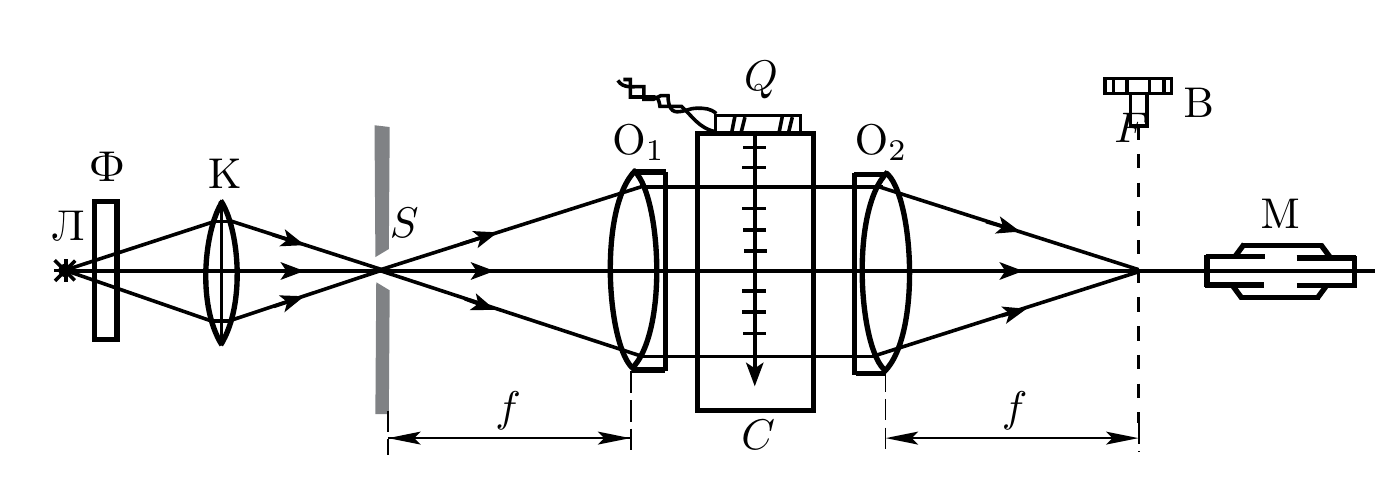
\includegraphics[scale=0.3]{schema_1.png}
    \caption{Схема устновки для измерений по дфиракционной картине}
\end{figure}

\noindent
После юстировки установки, меняя частоту генератора, дождемся появления дифракционных полос, видимых в микроскоп. 

\noindent
Измерим положение дифракционных полос $Y_m$ в зависимости от номера полосы. Повторим измерения для нескольких частот, на которых видна дифракционная картина. Результаты занесем в табл. 1.

\begin{table}[H]
    \centering
    \caption{Координаты дифракционных максимумов при различных частотах}
    \resizebox{18cm}{!}{
    \begin{tabular}{|c|c|c|c|c|c|c|c|} \hline
        $\nu = 1.080$ МГц & & $\nu = 1.936$ МГц & & $\nu = 3.219$ МГц & & $\nu = 4.430$ МГц & \\ \hline
        $m$ & $x_m$, мкм & $m$ & $x_m$, мкм & $m$ & $x_m$, мкм & $m$ & $x_m$, мкм \\ \hline
        -3 & -144 & -2 & 152 & -1 & 264 &-1 & 16 \\ \hline 
        -2 & -28 & -1 & 412 & 0 & 640 & 0&560  \\ \hline
        -1 & 92 & 0 & 628 & 1 & 1008  & 1 &1076 \\ \hline
        0 & 228 & 1 & 852 & --- & --- & ---&---  \\ \hline
        1 & 368 & 2 & 1100 & --- &--- & ---&---  \\ \hline
        2 & 488 & ---& ---& ---&--- & ---&--- \\ \hline
        3 & 604 &--- &--- &--- &--- & ---&---  \\ \hline
    \end{tabular}
}
\end{table}

\noindent
По результам измерений построим графики, представленные на рис. 3. Здесь $\Delta x_m = l_m$ -- расстояние от нулевого максимума до $m$-того максимума.

\begin{figure}[H]
    \centering
    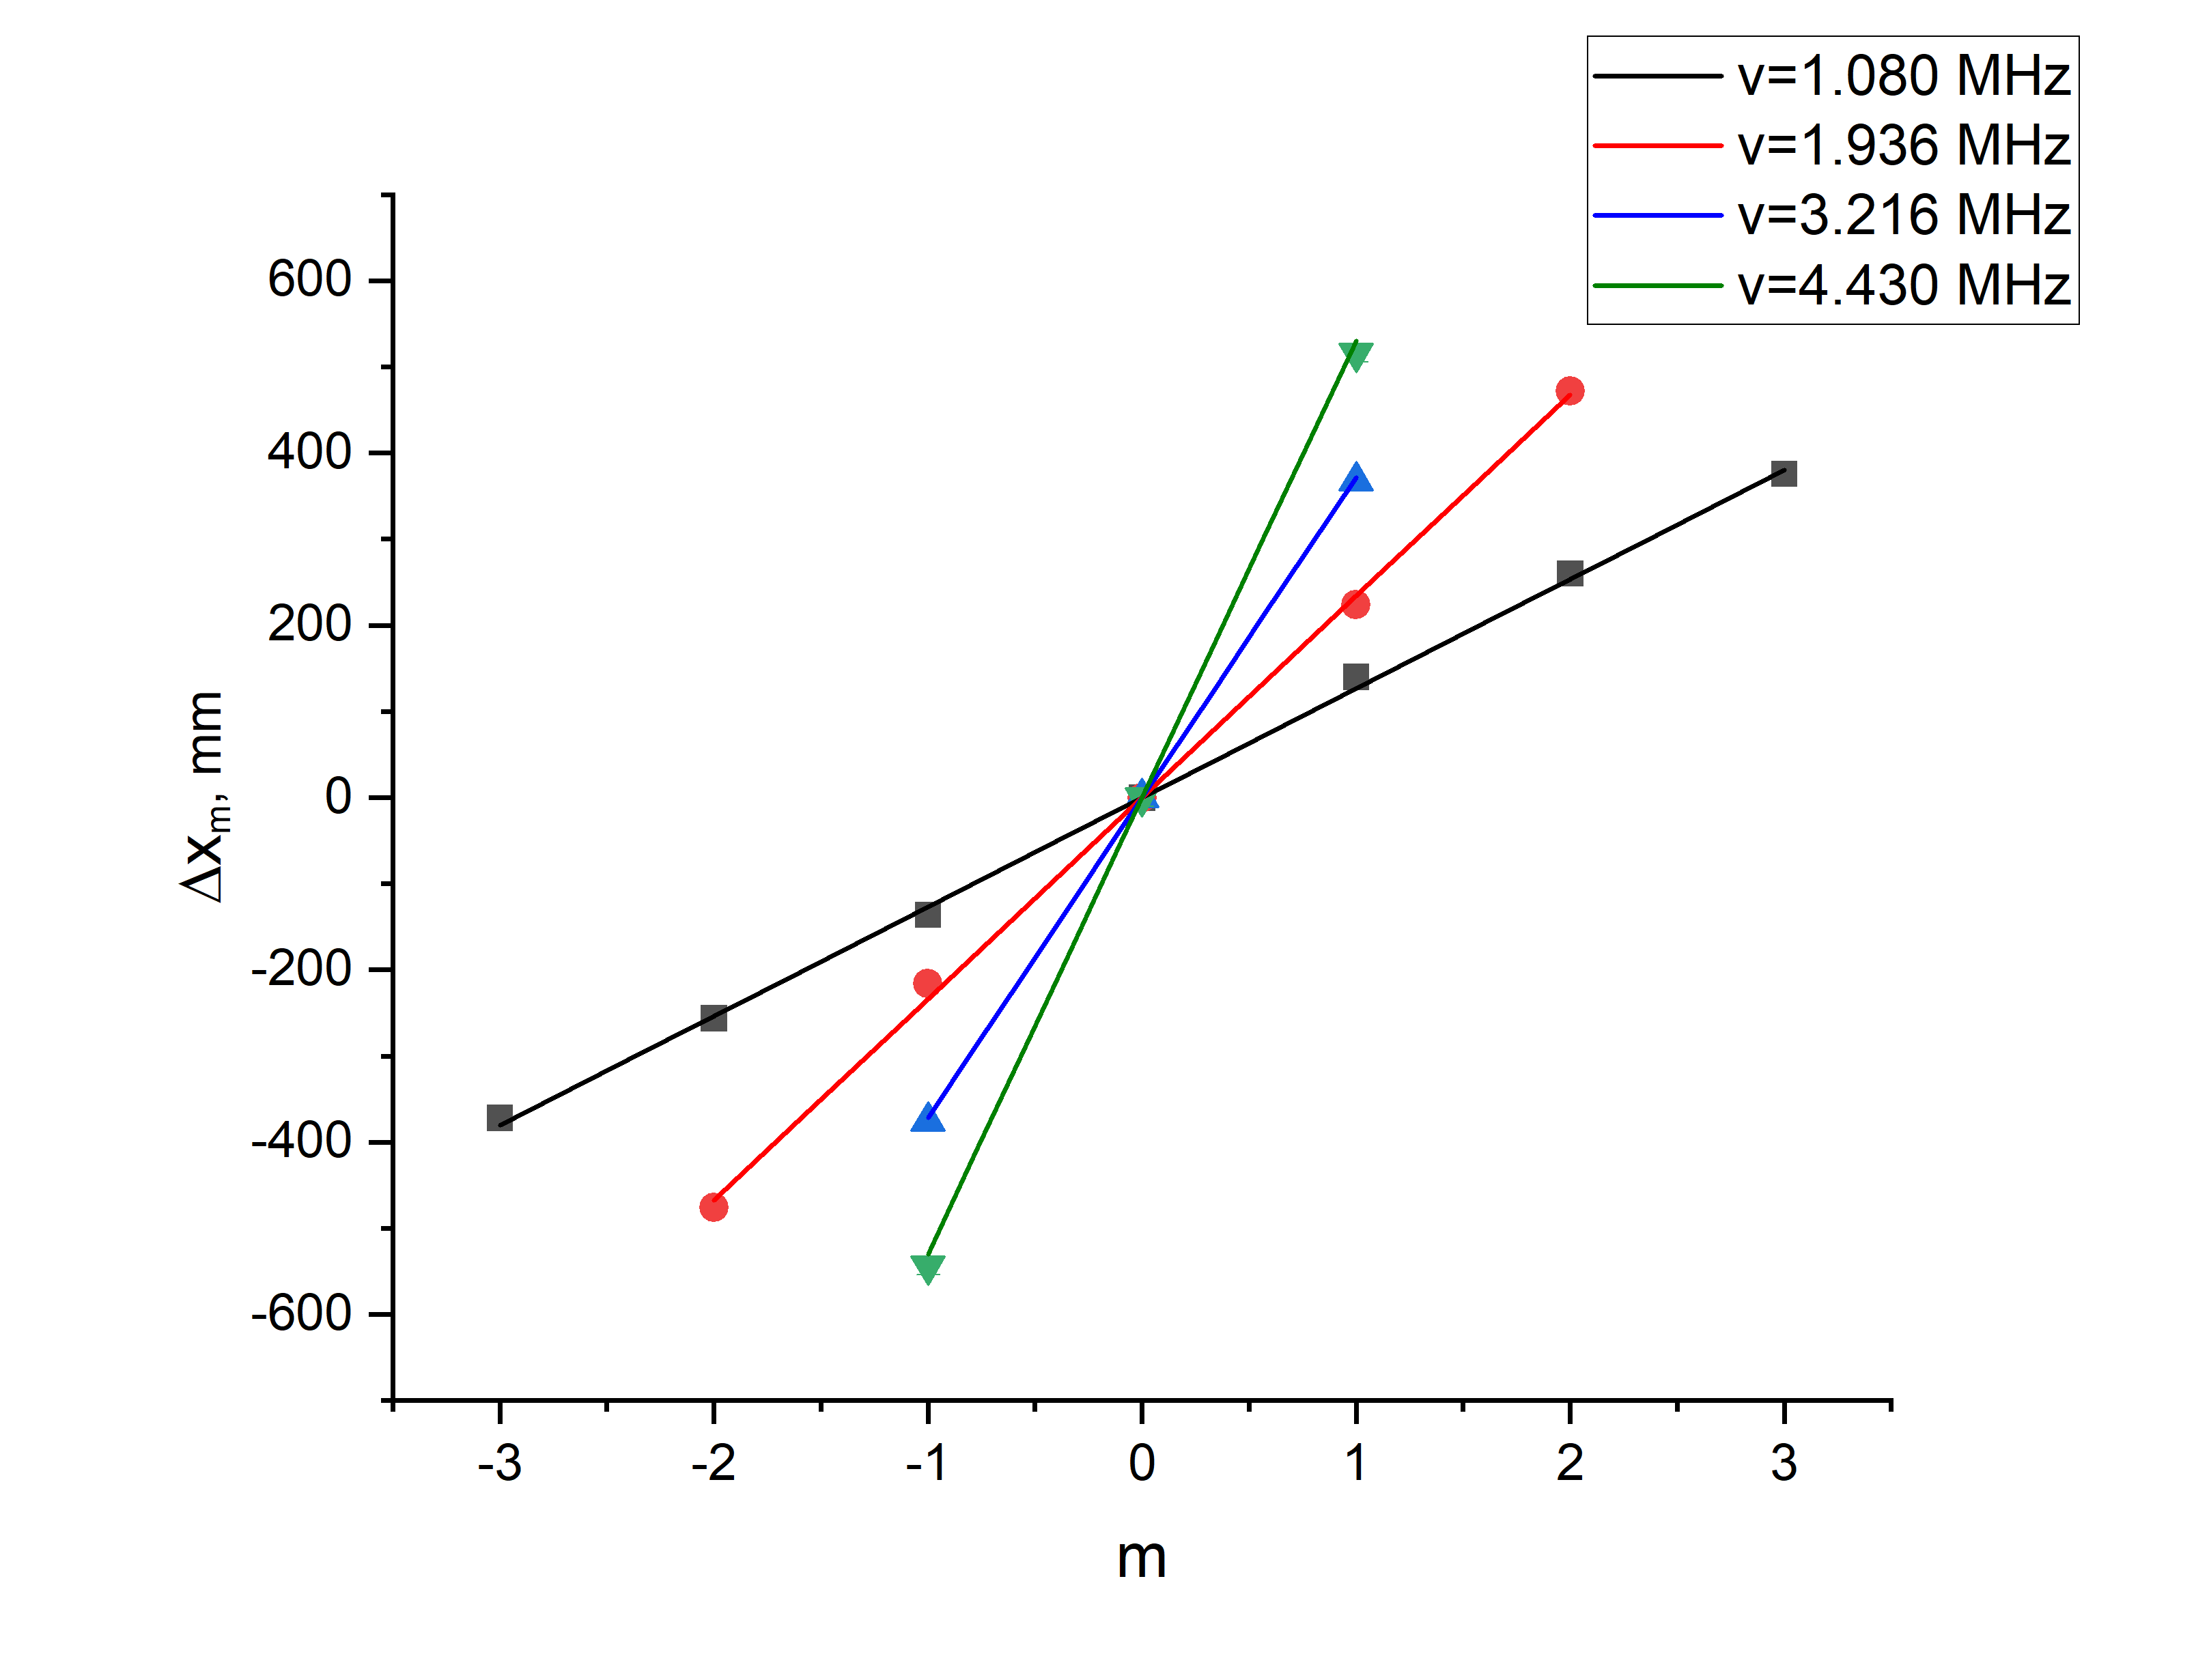
\includegraphics[scale=0.55]{1.png}
    \caption{Зависимость расстояния между максимумами от номера}
\end{figure}

\noindent
Из графика получаем коэффициенты наклона $l_m / m$. Затем, пользуюсь формулами (3) и (4), получаем длину волны и скорость ультразвука. Результаты в табл. 2.

\begin{table}[H]
    \centering
    \caption{Длина волны и скорость ультразвука}
    \begin{tabular}{|c|c|c|c|} \hline
        $\nu$, МГц & $\l_m / m$, мкм & $\Lambda$, мм & $v$, м/с  \\ \hline
        1.080 & 126.86 & 1.41 & 1525 \\ \hline
        1.936 & 233.61 & 0.77 & 1489 \\ \hline
        3.216 & 372.00 & 0.48 & 1550 \\ \hline
        4.430 & 530.00 & 0.34 & 1506\\ \hline
    \end{tabular}
\end{table}

\noindent
Отсюда среднее значение $v = 1518$ м/с.

\paragraph{Определение скорости ультразвука методом темного поля}
\n
Для измерений методом темного поля добавим к системе еще одну линзу, расположив ее между микроскопом и линзой O$_2$. Затем настроим микроскоп на резкое изображение сетки и премещая добавленную линзу добьемся того, чтобы блыи видны горизонтальные и вертикальные штрихи сетки. Затем закроим нулевой максимум щелью (положение нити, необходимое для этого было установлено в прошлой части работы). Меняя частоту, наблюдаем акустическую решетку. Измерим для различных частот расстояние координаты крайних хоршо видимымиых темных полом и число светлых промежутков между ними. Также рассчитаем, использую измерения, длину волны по формуле $\Lambda = 2 * (x_1 - x_0) / m$. Результаты в табл. 3.

\begin{table}[H]
    \centering
    \caption{Измерения методом темного поля}
    \begin{tabular}{|c|c|c|c|c|} \hline
        $\nu$, Мгц & $x_0$, мм & $x_1$, мм & $m$ & $\Lambda$, мм \\ \hline
        1.1459 & 5.0 & 6.4 & 2 & 1.40 \\ \hline
        1.2235 & 4.8 & 6.0 & 2 & 1.20 \\ \hline
        1.5673 & 4.4 & 5.8 & 3 & 0.93 \\ \hline
        2.0148 & 5.0 & 6.0 & 3 & 0.67 \\ \hline
        2.1216 & 4.7 & 6.0 & 4 & 0.65 \\ \hline
    \end{tabular}
\end{table}

\noindent
Построи теперь график зависимости $\Lambda$ от $1/\nu$ (рис. 4). По нему можем определить скорость ультразвука $v = 1790	 \pm 110$ м/с. 

\begin{figure}[H]
    \centering
    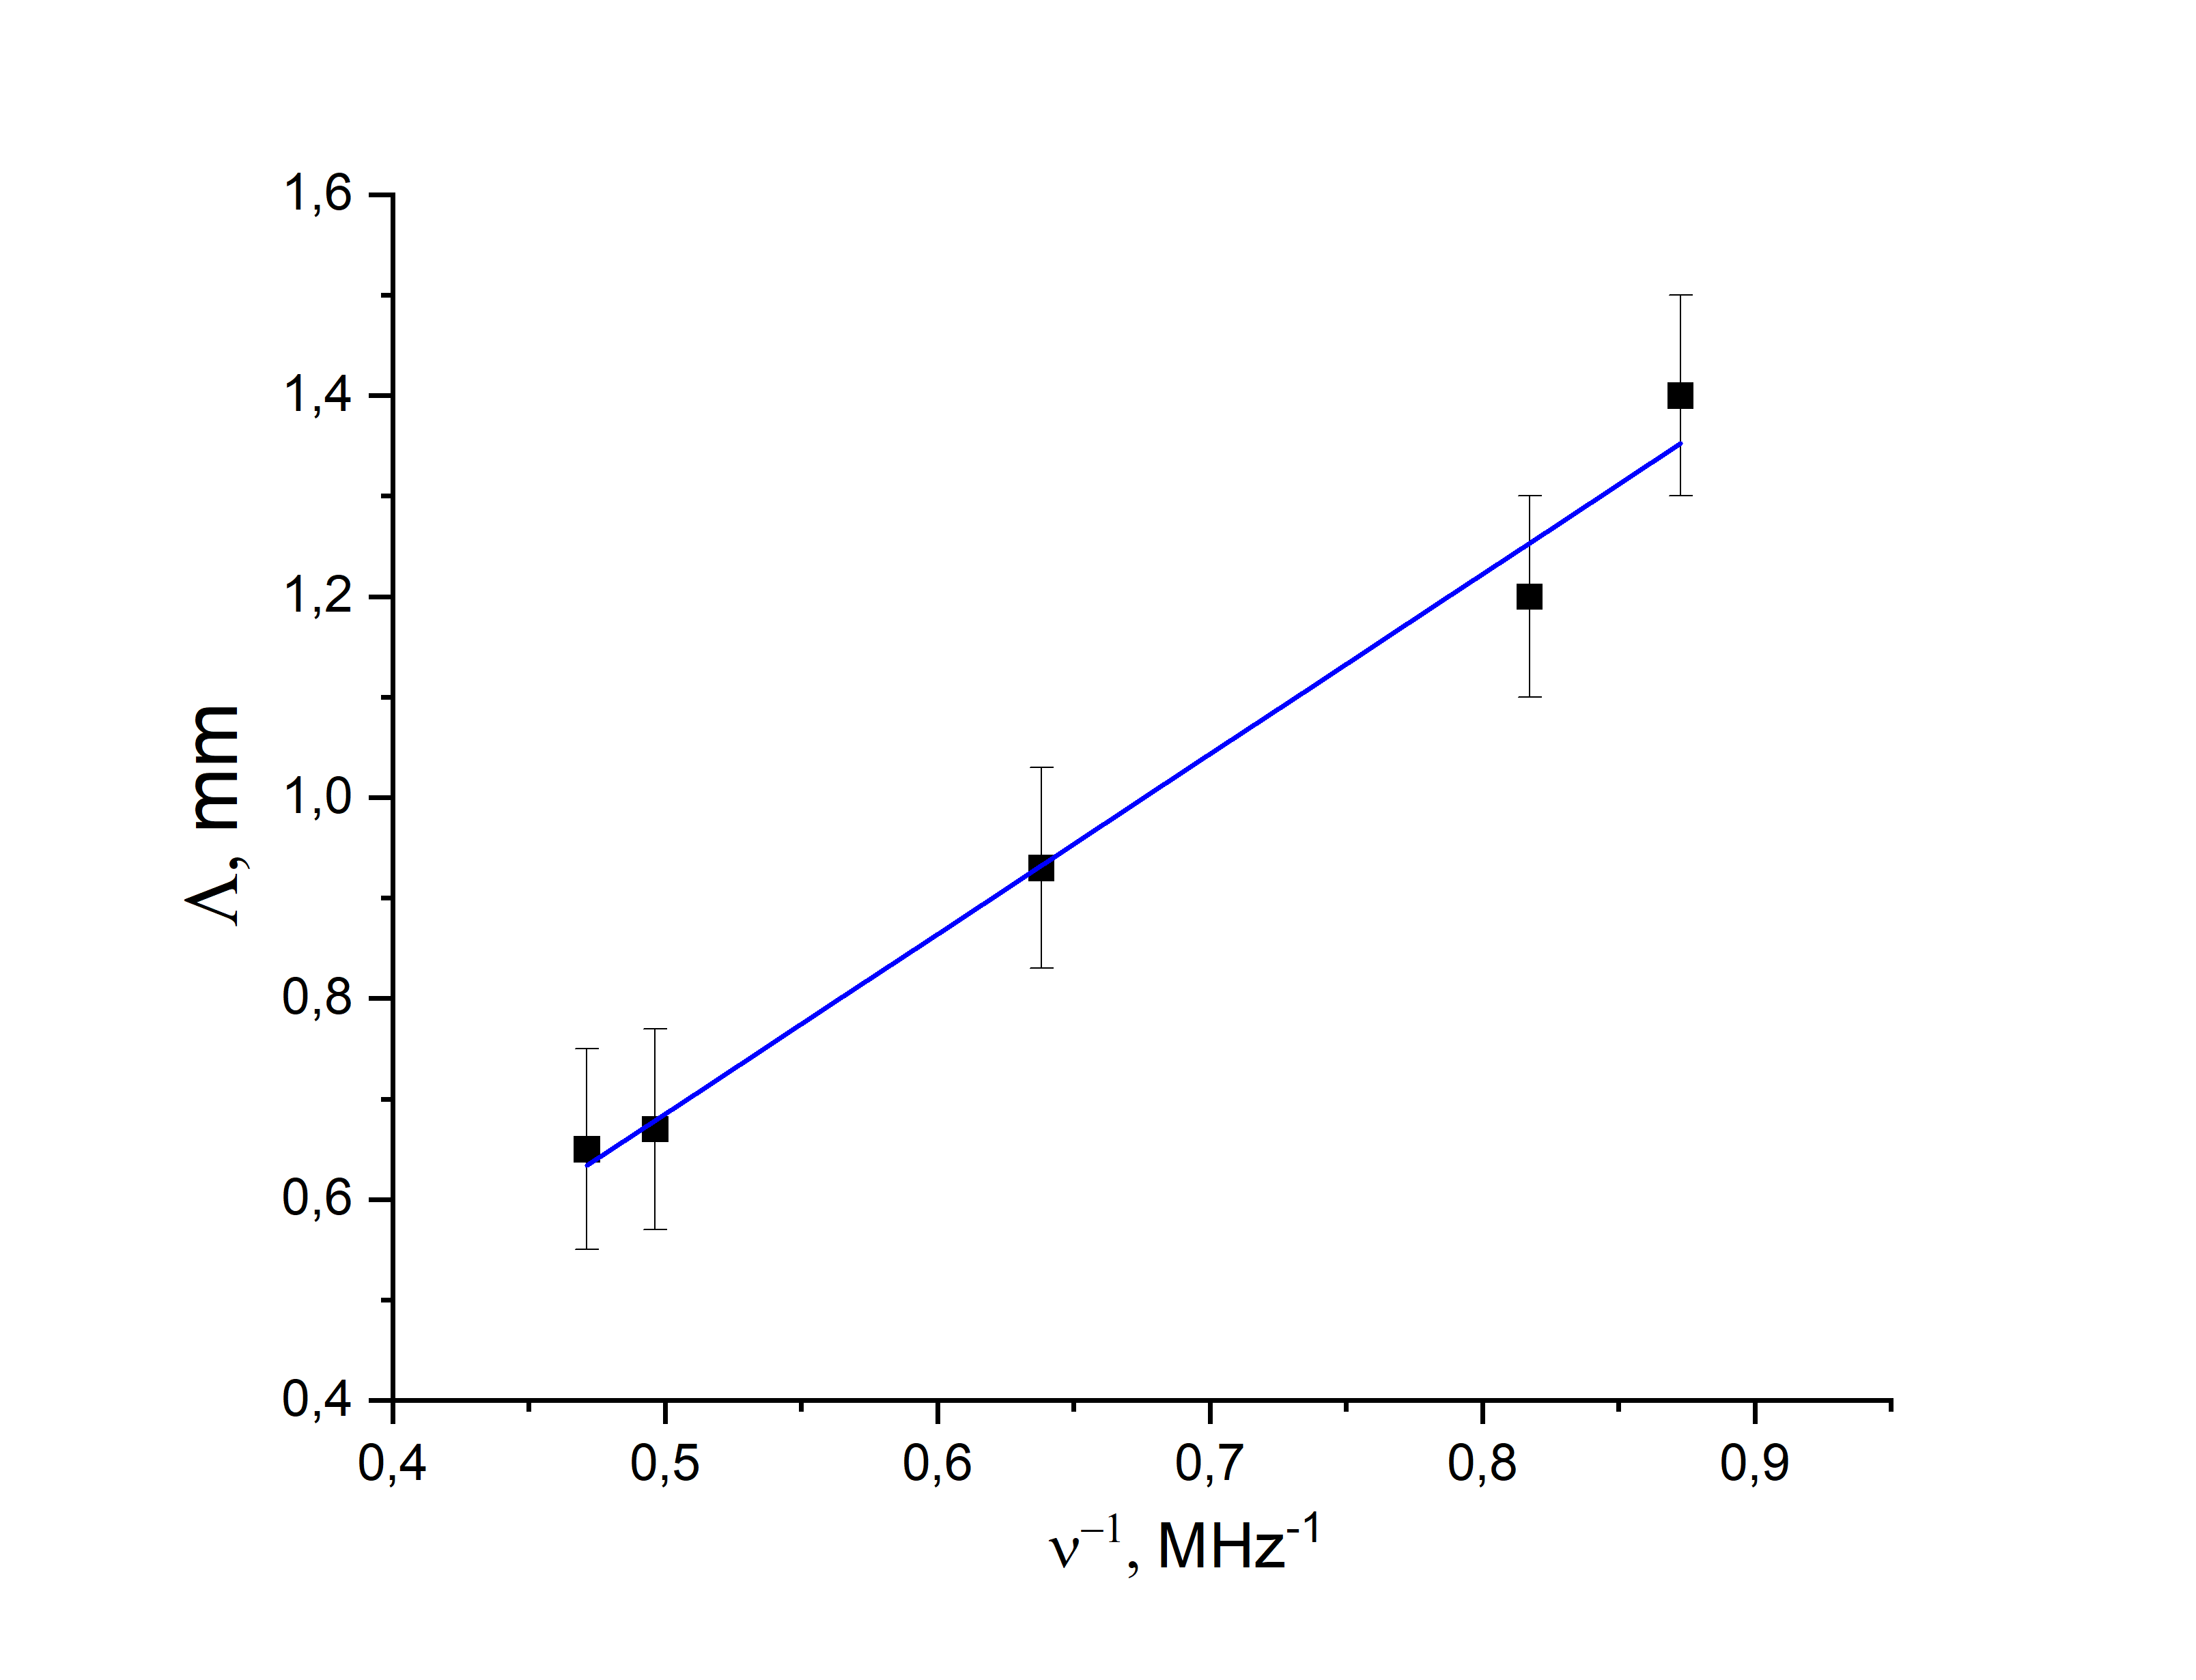
\includegraphics[scale=0.55]{2.png}
    \caption{Зависимости $\Lambda$ от $1/\nu$}
\end{figure}

\paragraph{Качественные наблюдения}
\n
При закрытии проволкой максимума с номером, отличным от 0, наблюдаем, что период картины не меняется, а менется лишь четкость картины. Это связано с тем, что на период на период влиет лишь расстояние между ближайшими максимума, которые формируют эту картину, а при закрытии одного любого из них, расстояние между ближайшими не меняется.

\pagebreak

\section*{Заключение}
Были проведены измерения скорости ультразвука двумя разными способами:
\begin{enumerate}
    \item По дифракционной картине. Получены значения $v = 1525$ м/с, $v = 1489$ м/с, $v = 1550$ м/с, $v = 1506$ м/с и среднее $v = 1518$ м/с.
    \item Измерения методом темного поля. Получено значение $v = (179 \pm 11) \cdot 10 $ м/с.
\end{enumerate}
Видим, что значение, полученное методом темного поля, не сходится в пределах погрешности со средним значением, как и не сходится с некоторыми отдельными значениями. Это может объясняться тем, что при измерении по дифракционной картине относительно велика погрешность измерений, так как эти измерения основываются на измерениях расстояния между дифракционными максимумами, расстояние между которыми может быть неверно измерено из-за мелкости измеряемой картины. Тем не менее, полученное значение можно считать приемлимым.

\end{document}

